\begin{frame}
    \frametitle{Большое левое вращение}

    %картинка 2
    \begin{figure}[ht]
        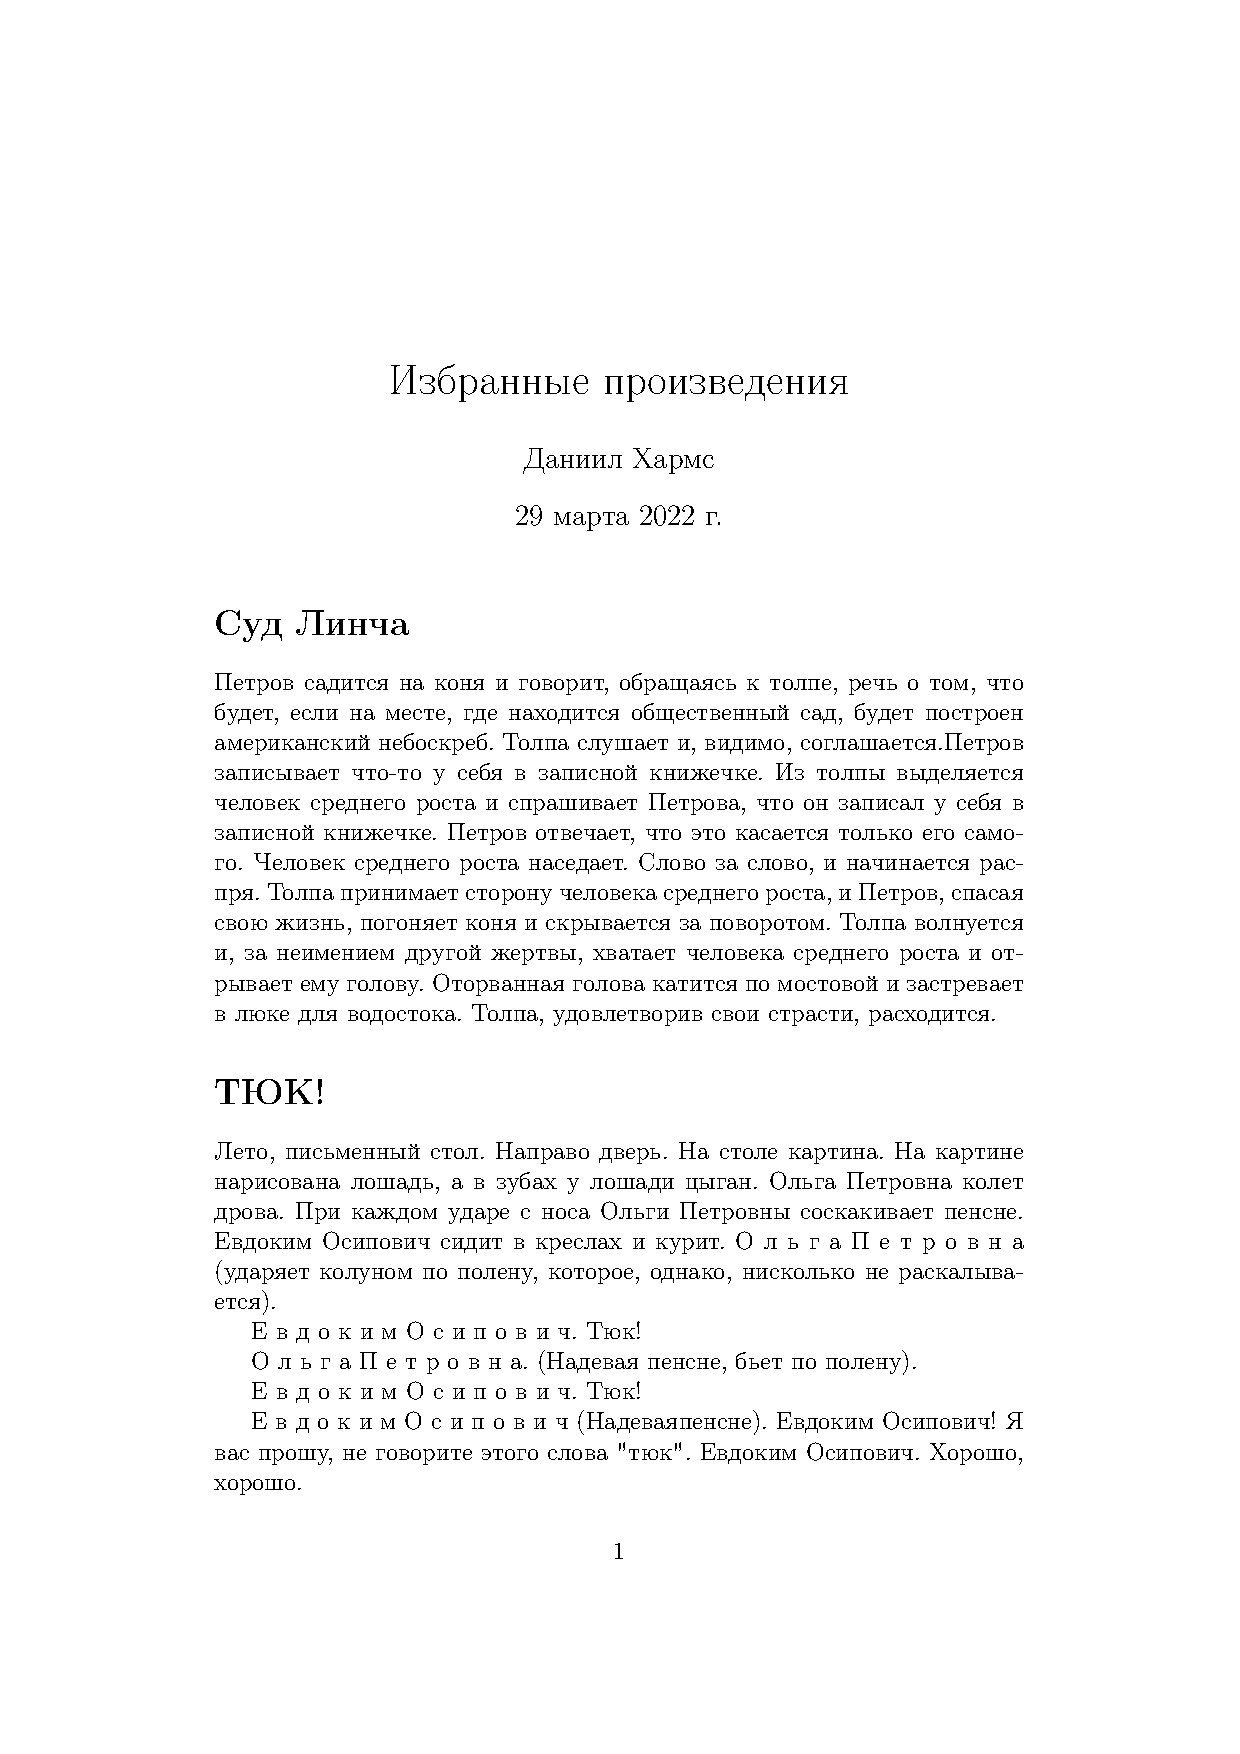
\includegraphics[width = \textwidth]{./images/2.pdf}

        \caption{Схематическое изображение большого левого вращения}
    \end{figure}

    Данное вращение используется тогда,
    когда (высота $b$"=поддерева; $L$ "--- высота)
    $= 2$ и высота $c$"=поддерева $>$ высота $R$.
\end{frame}